\subsection{Central Neutron Detector (CND)}

The CND geometry is implemented through the native GEMC geometry API. The paddles are Geant4 generic trapezoids
(see \F{cndGeometry}). The U-turn light guides are Geant4 ``polycones'' (volumes with cylindrical symmetry with varying
radius along one axis). The paddles are assigned the scintillator material and associated with the CND hit process routine.

\begin{figure}
	\centering
	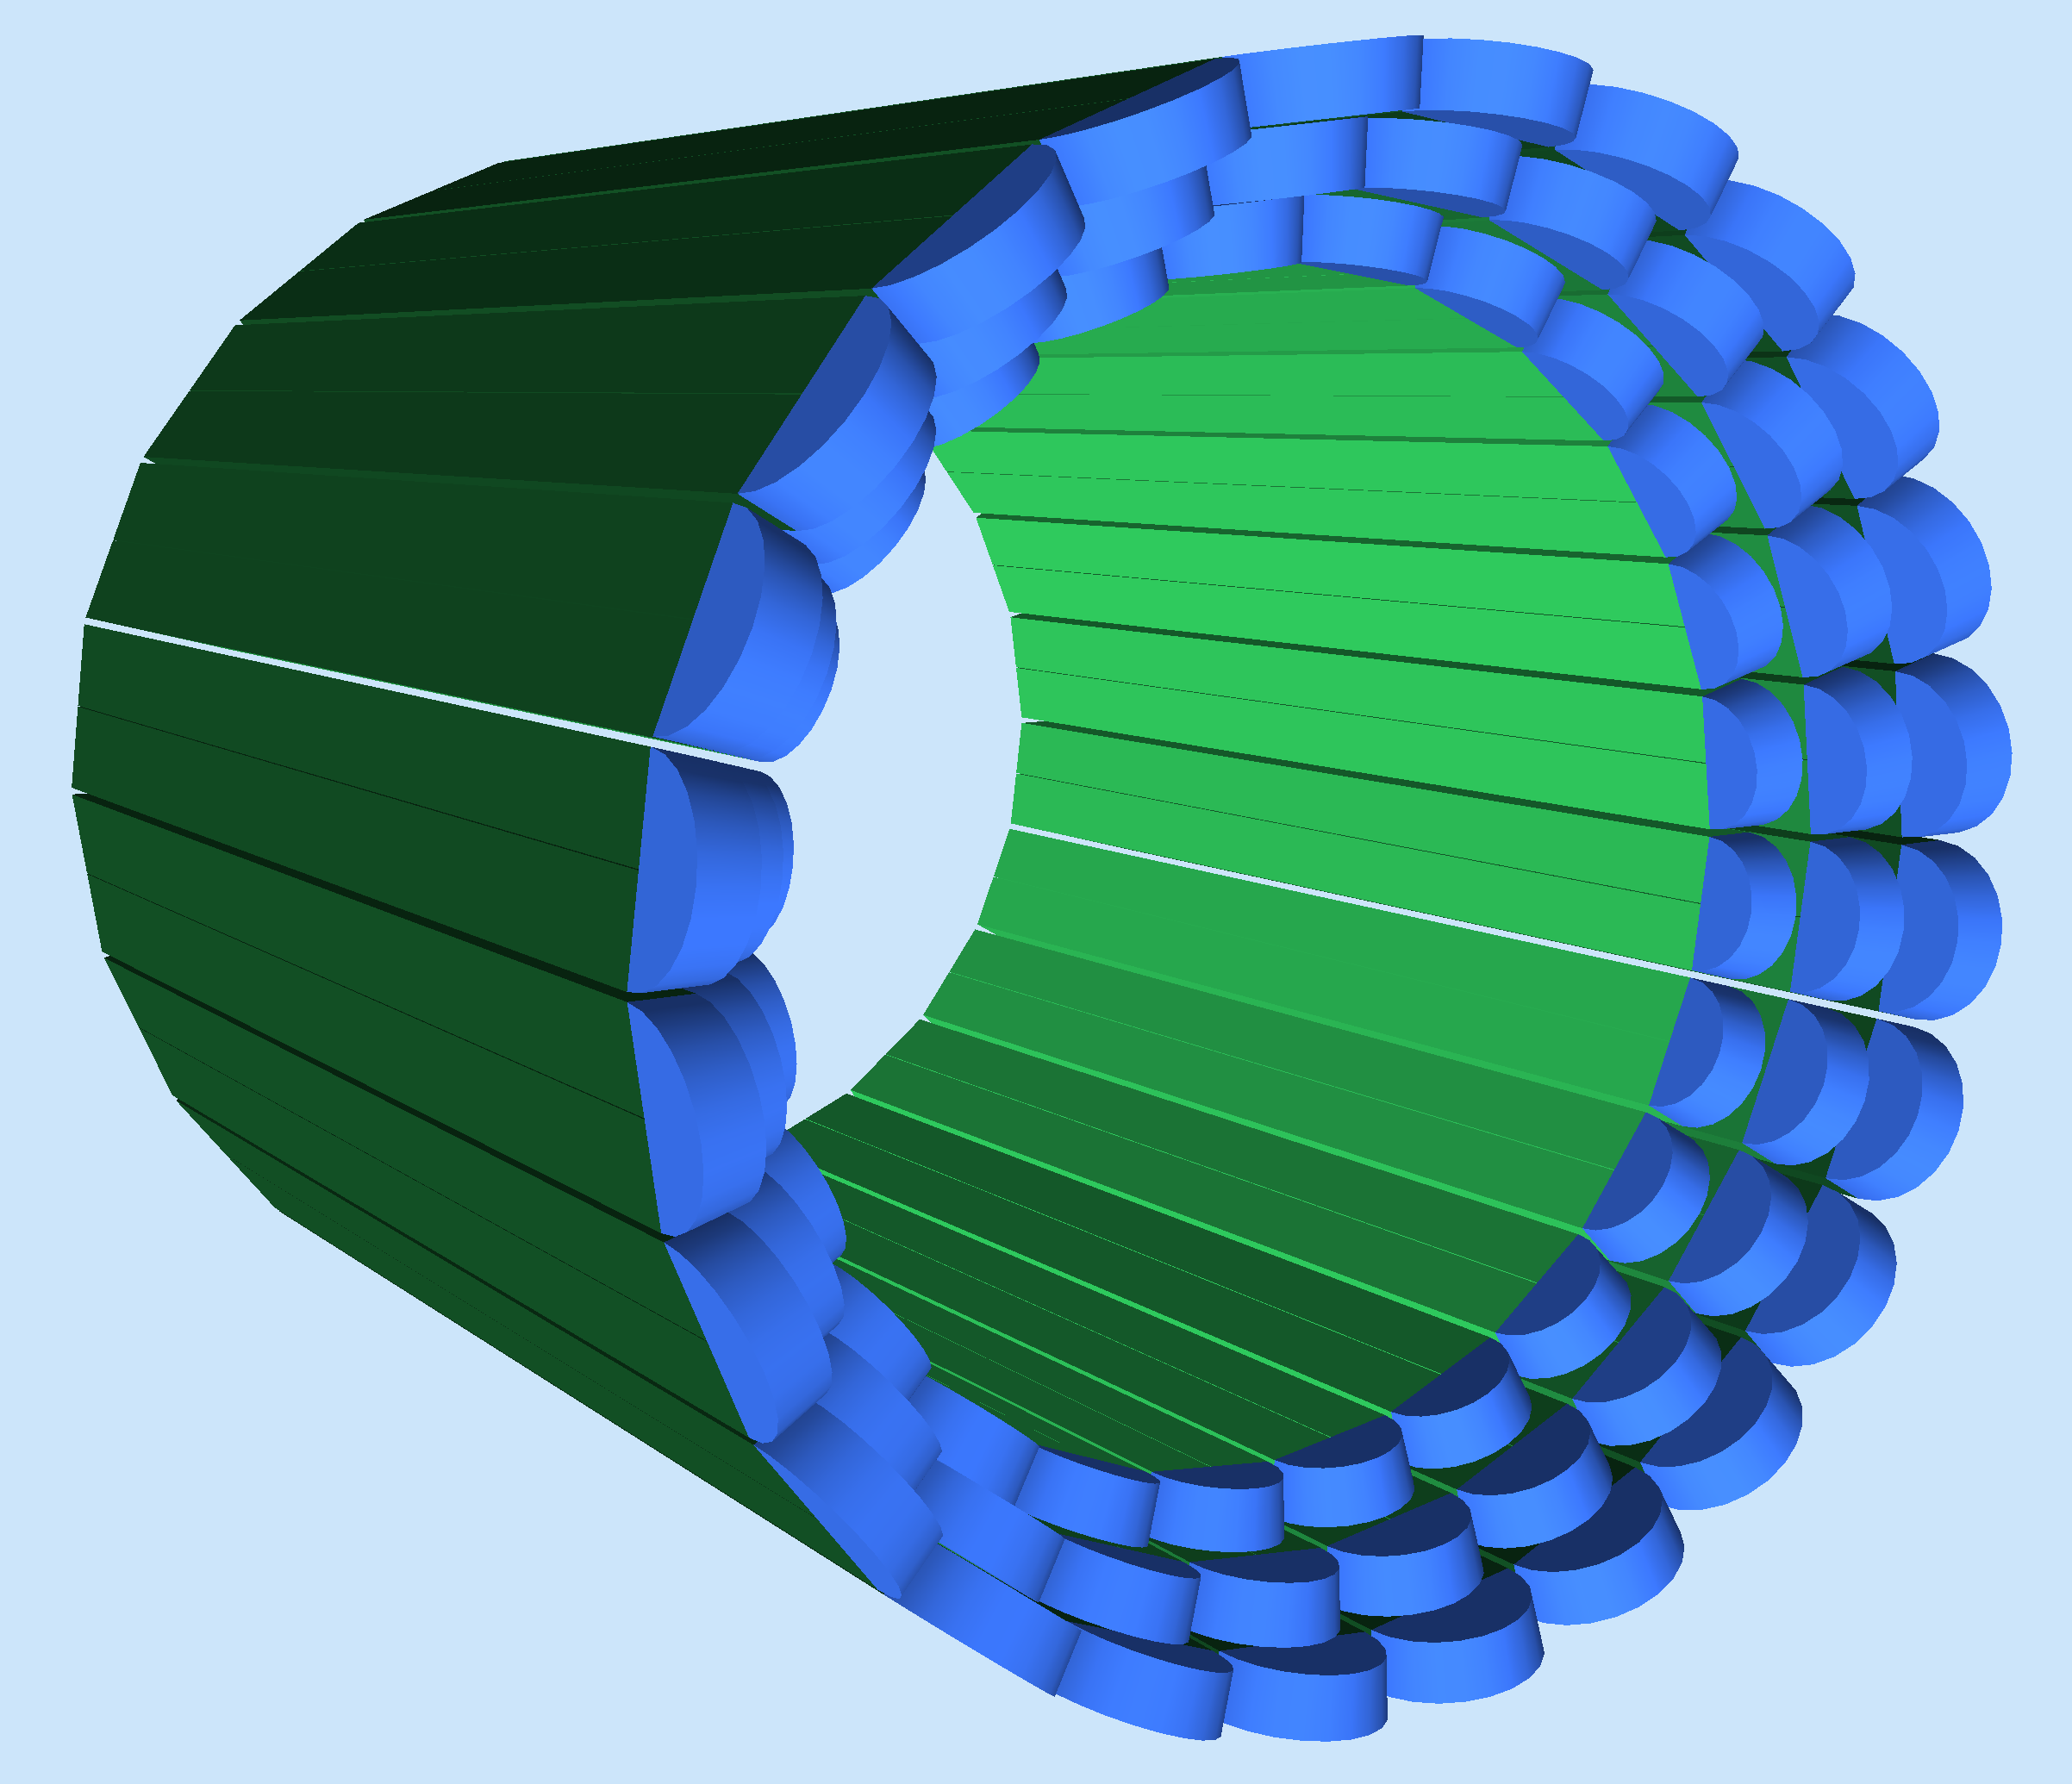
\includegraphics[width=0.99\columnwidth,keepaspectratio]{img/cndGeometry.png}
	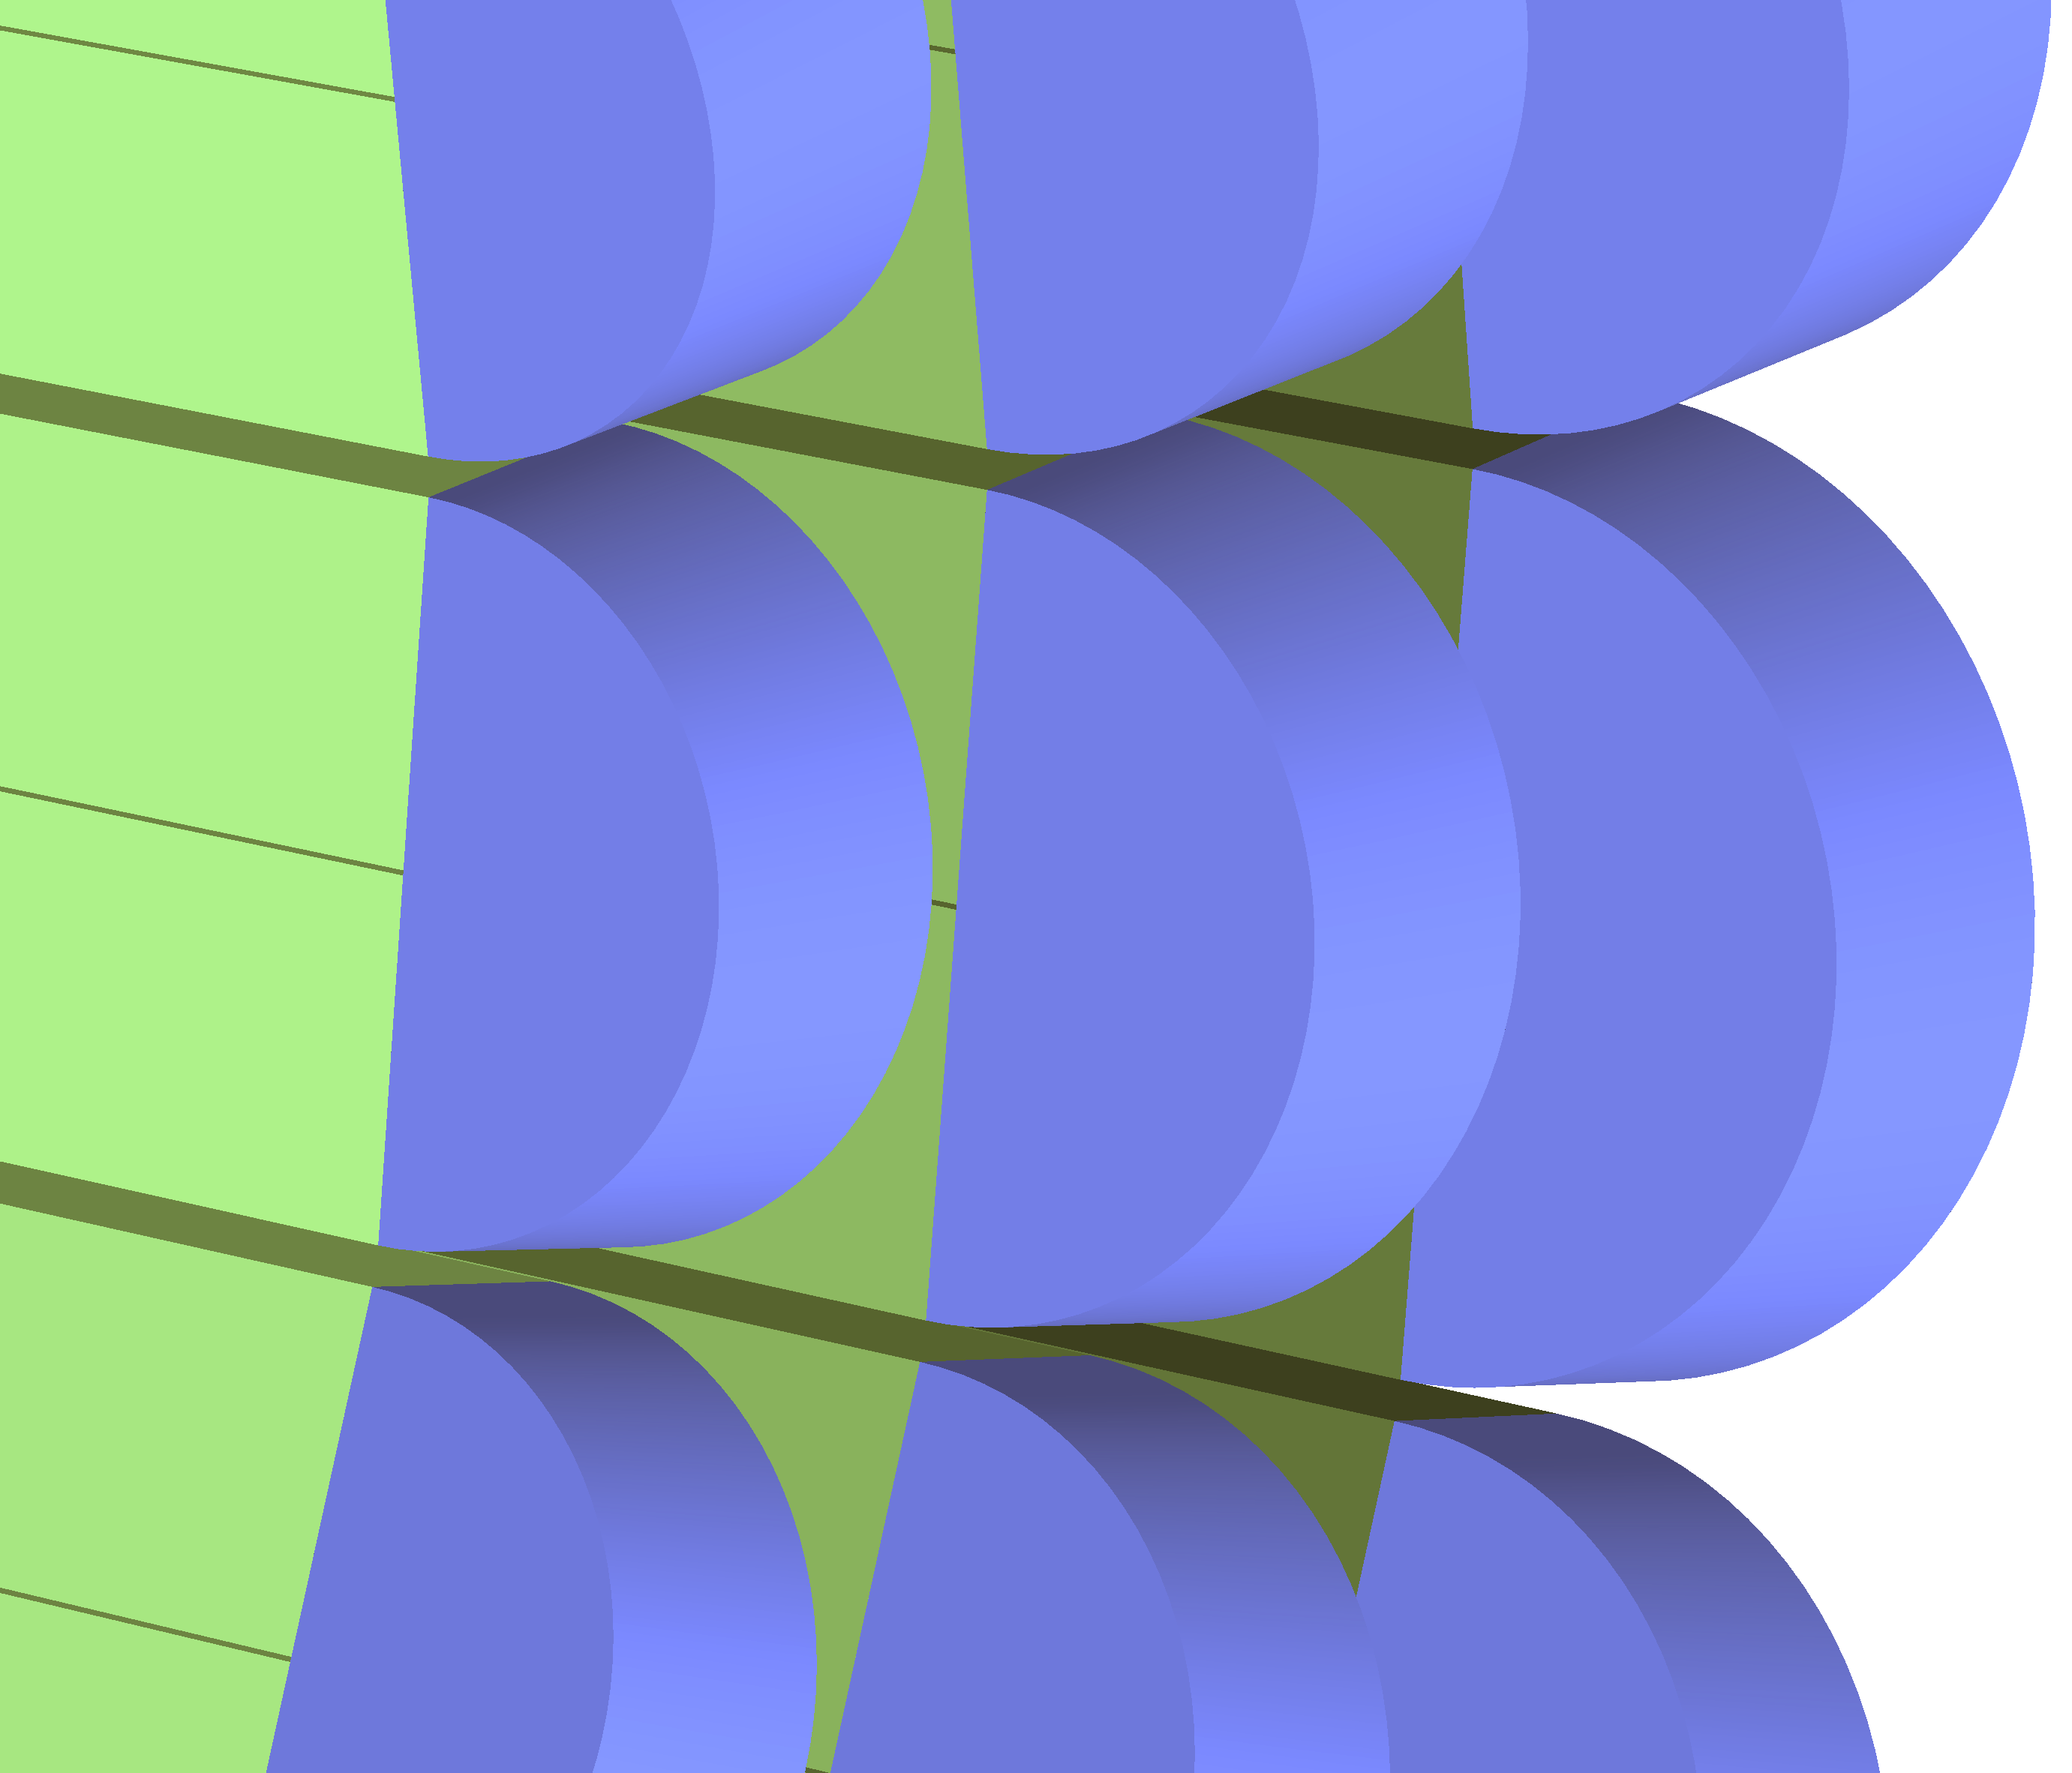
\includegraphics[width=0.99\columnwidth,keepaspectratio]{img/cndDetail.png}
	\caption{Top: overall view of the CND detector. Beam is incident from the left.
	         Three layers of scintillator are placed at increasing $z$. Pairs of scintillators
             are connected through a scintillator u-turn junction. Bottom: enlarged view of the junctions. }
	\label{fig:cndGeometry}
\end{figure}

\subsubsection{Digitization}

The energy deposited is reduced based on the position in the paddle using the calibrated light attenuation length.
Two signals are then propagated, one to the PMT attached to the scintillator (``direct hit''), and one traveling
through the scintillator junction onto the other scintillator and its PMT (``indirect hit''). Layer-dependent factors,
applied to the two  signals, account for the light loss in the U-turn and in the neighboring paddle. These factors were
determined during cosmic-ray tests.

The corrected energy is converted to the theoretical number of photons $N_{th}$ using the constant 1210~$\gamma$/MeV,
which accounts for light propagation in the 1.4-m-long light guides, for losses at the junctions and for the quantum
efficiency of the PMT. A Poissonian distribution is used to calculate the actual number of photons $N_{actual}$ and the
resulting ``smeared'' energy is then converted to ADC using the FADC conversion factor.

The absolute hit time is corrected using calibration constants estimated from data:

\begin{itemize}
	\item the effective velocity;
	\item a left/right time offset factor;
	\item the Birks-attenuation factor;
	\item the position and corresponding paddle length of the direct and the indirect hit.
\end{itemize}

The time is then smeared by a resolution read from CCDB using a Gaussian function and then digitized using a TDC
conversion factor. The Birks factor, reducing the deposited energy depending on the particle type, enters in the timing
calculation as follows: the direct and indirect times are smeared with a Gaussian function having a width directly
proportional to an empirically determined constant, and inversely proportional to the square root of the measured
light (which is, in turn, proportional to the attenuated energy). The digitized output bank variables are summarized in
Table~\ref{tab:cndBank}.

\begin{table}[h]
	\begin{center}
		\begin{tabular}{| c | c | c |}
			\hline \hline
			Variable  &          Description     \\
			\hline
              sector  &        sector number     \\
               layer  &         layer number     \\
           component  &     component number     \\
                ADCL  &             ADC Left     \\
                ADCR  &            ADC Right     \\
                TDCL  &             TDC Left     \\
                TDCR  &            TDC Right     \\
                hitn  &           hit number     \\
			\hline \hline
		\end{tabular}
	\end{center}
	\caption{The digitized CND bank.}\label{tab:cndBank}
\end{table}

The time window  of the CND is set to 400~ns: all Geant4 steps within the same paddle and time window are collected
in one hit.
